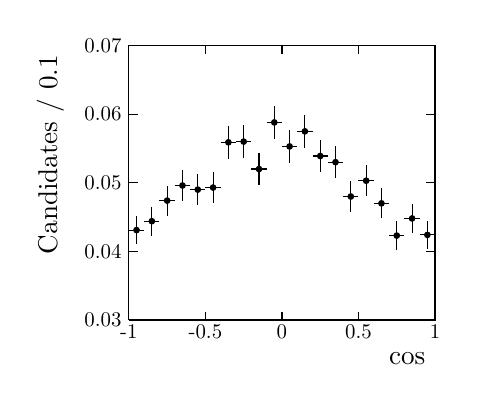
\begin{tikzpicture}
\pgfdeclareplotmark{cross} {
\pgfpathmoveto{\pgfpoint{-0.3\pgfplotmarksize}{\pgfplotmarksize}}
\pgfpathlineto{\pgfpoint{+0.3\pgfplotmarksize}{\pgfplotmarksize}}
\pgfpathlineto{\pgfpoint{+0.3\pgfplotmarksize}{0.3\pgfplotmarksize}}
\pgfpathlineto{\pgfpoint{+1\pgfplotmarksize}{0.3\pgfplotmarksize}}
\pgfpathlineto{\pgfpoint{+1\pgfplotmarksize}{-0.3\pgfplotmarksize}}
\pgfpathlineto{\pgfpoint{+0.3\pgfplotmarksize}{-0.3\pgfplotmarksize}}
\pgfpathlineto{\pgfpoint{+0.3\pgfplotmarksize}{-1.\pgfplotmarksize}}
\pgfpathlineto{\pgfpoint{-0.3\pgfplotmarksize}{-1.\pgfplotmarksize}}
\pgfpathlineto{\pgfpoint{-0.3\pgfplotmarksize}{-0.3\pgfplotmarksize}}
\pgfpathlineto{\pgfpoint{-1.\pgfplotmarksize}{-0.3\pgfplotmarksize}}
\pgfpathlineto{\pgfpoint{-1.\pgfplotmarksize}{0.3\pgfplotmarksize}}
\pgfpathlineto{\pgfpoint{-0.3\pgfplotmarksize}{0.3\pgfplotmarksize}}
\pgfpathclose
\pgfusepathqstroke
}
\pgfdeclareplotmark{cross*} {
\pgfpathmoveto{\pgfpoint{-0.3\pgfplotmarksize}{\pgfplotmarksize}}
\pgfpathlineto{\pgfpoint{+0.3\pgfplotmarksize}{\pgfplotmarksize}}
\pgfpathlineto{\pgfpoint{+0.3\pgfplotmarksize}{0.3\pgfplotmarksize}}
\pgfpathlineto{\pgfpoint{+1\pgfplotmarksize}{0.3\pgfplotmarksize}}
\pgfpathlineto{\pgfpoint{+1\pgfplotmarksize}{-0.3\pgfplotmarksize}}
\pgfpathlineto{\pgfpoint{+0.3\pgfplotmarksize}{-0.3\pgfplotmarksize}}
\pgfpathlineto{\pgfpoint{+0.3\pgfplotmarksize}{-1.\pgfplotmarksize}}
\pgfpathlineto{\pgfpoint{-0.3\pgfplotmarksize}{-1.\pgfplotmarksize}}
\pgfpathlineto{\pgfpoint{-0.3\pgfplotmarksize}{-0.3\pgfplotmarksize}}
\pgfpathlineto{\pgfpoint{-1.\pgfplotmarksize}{-0.3\pgfplotmarksize}}
\pgfpathlineto{\pgfpoint{-1.\pgfplotmarksize}{0.3\pgfplotmarksize}}
\pgfpathlineto{\pgfpoint{-0.3\pgfplotmarksize}{0.3\pgfplotmarksize}}
\pgfpathclose
\pgfusepathqfillstroke
}
\pgfdeclareplotmark{newstar} {
\pgfpathmoveto{\pgfqpoint{0pt}{\pgfplotmarksize}}
\pgfpathlineto{\pgfqpointpolar{44}{0.5\pgfplotmarksize}}
\pgfpathlineto{\pgfqpointpolar{18}{\pgfplotmarksize}}
\pgfpathlineto{\pgfqpointpolar{-20}{0.5\pgfplotmarksize}}
\pgfpathlineto{\pgfqpointpolar{-54}{\pgfplotmarksize}}
\pgfpathlineto{\pgfqpointpolar{-90}{0.5\pgfplotmarksize}}
\pgfpathlineto{\pgfqpointpolar{234}{\pgfplotmarksize}}
\pgfpathlineto{\pgfqpointpolar{198}{0.5\pgfplotmarksize}}
\pgfpathlineto{\pgfqpointpolar{162}{\pgfplotmarksize}}
\pgfpathlineto{\pgfqpointpolar{134}{0.5\pgfplotmarksize}}
\pgfpathclose
\pgfusepathqstroke
}
\pgfdeclareplotmark{newstar*} {
\pgfpathmoveto{\pgfqpoint{0pt}{\pgfplotmarksize}}
\pgfpathlineto{\pgfqpointpolar{44}{0.5\pgfplotmarksize}}
\pgfpathlineto{\pgfqpointpolar{18}{\pgfplotmarksize}}
\pgfpathlineto{\pgfqpointpolar{-20}{0.5\pgfplotmarksize}}
\pgfpathlineto{\pgfqpointpolar{-54}{\pgfplotmarksize}}
\pgfpathlineto{\pgfqpointpolar{-90}{0.5\pgfplotmarksize}}
\pgfpathlineto{\pgfqpointpolar{234}{\pgfplotmarksize}}
\pgfpathlineto{\pgfqpointpolar{198}{0.5\pgfplotmarksize}}
\pgfpathlineto{\pgfqpointpolar{162}{\pgfplotmarksize}}
\pgfpathlineto{\pgfqpointpolar{134}{0.5\pgfplotmarksize}}
\pgfpathclose
\pgfusepathqfillstroke
}
\definecolor{c}{rgb}{1,1,1};
\draw [color=c, fill=c] (0.1,4.68649) rectangle (4.9,9.0973);
\draw [color=c, fill=c] (0.772,5.39222) rectangle (4.66,8.87676);
\definecolor{c}{rgb}{0,0,0};
\draw [c] (0.772,5.39222) -- (0.772,8.87676) -- (4.66,8.87676) -- (4.66,5.39222) -- (0.772,5.39222);
\draw [c,line width=0.4] (0.8692,6.35255) -- (0.8692,6.5334);
\draw [c,line width=0.4] (0.8692,6.5334) -- (0.8692,6.71426);
\draw [c,line width=0.4] (0.772,6.5334) -- (0.8692,6.5334);
\draw [c,line width=0.4] (0.8692,6.5334) -- (0.9664,6.5334);
\foreach \P in {(0.8692,6.5334)}{\draw[mark options={color=c,fill=c},mark size=1.201201pt,mark=*,mark size=1pt] plot coordinates {\P};}
\draw [c,line width=0.4] (1.0636,6.46309) -- (1.0636,6.64665);
\draw [c,line width=0.4] (1.0636,6.64665) -- (1.0636,6.83021);
\draw [c,line width=0.4] (0.9664,6.64665) -- (1.0636,6.64665);
\draw [c,line width=0.4] (1.0636,6.64665) -- (1.1608,6.64665);
\foreach \P in {(1.0636,6.64665)}{\draw[mark options={color=c,fill=c},mark size=1.201201pt,mark=*,mark size=1pt] plot coordinates {\P};}
\draw [c,line width=0.4] (1.258,6.71833) -- (1.258,6.90799);
\draw [c,line width=0.4] (1.258,6.90799) -- (1.258,7.09765);
\draw [c,line width=0.4] (1.1608,6.90799) -- (1.258,6.90799);
\draw [c,line width=0.4] (1.258,6.90799) -- (1.3552,6.90799);
\foreach \P in {(1.258,6.90799)}{\draw[mark options={color=c,fill=c},mark size=1.201201pt,mark=*,mark size=1pt] plot coordinates {\P};}
\draw [c,line width=0.4] (1.4524,6.90563) -- (1.4524,7.09964);
\draw [c,line width=0.4] (1.4524,7.09964) -- (1.4524,7.29365);
\draw [c,line width=0.4] (1.3552,7.09964) -- (1.4524,7.09964);
\draw [c,line width=0.4] (1.4524,7.09964) -- (1.5496,7.09964);
\foreach \P in {(1.4524,7.09964)}{\draw[mark options={color=c,fill=c},mark size=1.201201pt,mark=*,mark size=1pt] plot coordinates {\P};}
\draw [c,line width=0.4] (1.6468,6.85454) -- (1.6468,7.04737);
\draw [c,line width=0.4] (1.6468,7.04737) -- (1.6468,7.24021);
\draw [c,line width=0.4] (1.5496,7.04737) -- (1.6468,7.04737);
\draw [c,line width=0.4] (1.6468,7.04737) -- (1.744,7.04737);
\foreach \P in {(1.6468,7.04737)}{\draw[mark options={color=c,fill=c},mark size=1.201201pt,mark=*,mark size=1pt] plot coordinates {\P};}
\draw [c,line width=0.4] (1.8412,6.88008) -- (1.8412,7.07351);
\draw [c,line width=0.4] (1.8412,7.07351) -- (1.8412,7.26693);
\draw [c,line width=0.4] (1.744,7.07351) -- (1.8412,7.07351);
\draw [c,line width=0.4] (1.8412,7.07351) -- (1.9384,7.07351);
\foreach \P in {(1.8412,7.07351)}{\draw[mark options={color=c,fill=c},mark size=1.201201pt,mark=*,mark size=1pt] plot coordinates {\P};}
\draw [c,line width=0.4] (2.0356,7.44249) -- (2.0356,7.64846);
\draw [c,line width=0.4] (2.0356,7.64846) -- (2.0356,7.85442);
\draw [c,line width=0.4] (1.9384,7.64846) -- (2.0356,7.64846);
\draw [c,line width=0.4] (2.0356,7.64846) -- (2.1328,7.64846);
\foreach \P in {(2.0356,7.64846)}{\draw[mark options={color=c,fill=c},mark size=1.201201pt,mark=*,mark size=1pt] plot coordinates {\P};}
\draw [c,line width=0.4] (2.23,7.45102) -- (2.23,7.65717);
\draw [c,line width=0.4] (2.23,7.65717) -- (2.23,7.86332);
\draw [c,line width=0.4] (2.1328,7.65717) -- (2.23,7.65717);
\draw [c,line width=0.4] (2.23,7.65717) -- (2.3272,7.65717);
\foreach \P in {(2.23,7.65717)}{\draw[mark options={color=c,fill=c},mark size=1.201201pt,mark=*,mark size=1pt] plot coordinates {\P};}
\draw [c,line width=0.4] (2.4244,7.11006) -- (2.4244,7.30871);
\draw [c,line width=0.4] (2.4244,7.30871) -- (2.4244,7.50736);
\draw [c,line width=0.4] (2.3272,7.30871) -- (2.4244,7.30871);
\draw [c,line width=0.4] (2.4244,7.30871) -- (2.5216,7.30871);
\foreach \P in {(2.4244,7.30871)}{\draw[mark options={color=c,fill=c},mark size=1.201201pt,mark=*,mark size=1pt] plot coordinates {\P};}
\draw [c,line width=0.4] (2.6188,7.68985) -- (2.6188,7.90109);
\draw [c,line width=0.4] (2.6188,7.90109) -- (2.6188,8.11232);
\draw [c,line width=0.4] (2.5216,7.90109) -- (2.6188,7.90109);
\draw [c,line width=0.4] (2.6188,7.90109) -- (2.716,7.90109);
\foreach \P in {(2.6188,7.90109)}{\draw[mark options={color=c,fill=c},mark size=1.201201pt,mark=*,mark size=1pt] plot coordinates {\P};}
\draw [c,line width=0.4] (2.8132,7.39133) -- (2.8132,7.59619);
\draw [c,line width=0.4] (2.8132,7.59619) -- (2.8132,7.80104);
\draw [c,line width=0.4] (2.716,7.59619) -- (2.8132,7.59619);
\draw [c,line width=0.4] (2.8132,7.59619) -- (2.9104,7.59619);
\foreach \P in {(2.8132,7.59619)}{\draw[mark options={color=c,fill=c},mark size=1.201201pt,mark=*,mark size=1pt] plot coordinates {\P};}
\draw [c,line width=0.4] (3.0076,7.57895) -- (3.0076,7.78784);
\draw [c,line width=0.4] (3.0076,7.78784) -- (3.0076,7.99673);
\draw [c,line width=0.4] (2.9104,7.78784) -- (3.0076,7.78784);
\draw [c,line width=0.4] (3.0076,7.78784) -- (3.1048,7.78784);
\foreach \P in {(3.0076,7.78784)}{\draw[mark options={color=c,fill=c},mark size=1.201201pt,mark=*,mark size=1pt] plot coordinates {\P};}
\draw [c,line width=0.4] (3.202,7.27198) -- (3.202,7.47423);
\draw [c,line width=0.4] (3.202,7.47423) -- (3.202,7.67648);
\draw [c,line width=0.4] (3.1048,7.47423) -- (3.202,7.47423);
\draw [c,line width=0.4] (3.202,7.47423) -- (3.2992,7.47423);
\foreach \P in {(3.202,7.47423)}{\draw[mark options={color=c,fill=c},mark size=1.201201pt,mark=*,mark size=1pt] plot coordinates {\P};}
\draw [c,line width=0.4] (3.3964,7.19528) -- (3.3964,7.39583);
\draw [c,line width=0.4] (3.3964,7.39583) -- (3.3964,7.59638);
\draw [c,line width=0.4] (3.2992,7.39583) -- (3.3964,7.39583);
\draw [c,line width=0.4] (3.3964,7.39583) -- (3.4936,7.39583);
\foreach \P in {(3.3964,7.39583)}{\draw[mark options={color=c,fill=c},mark size=1.201201pt,mark=*,mark size=1pt] plot coordinates {\P};}
\draw [c,line width=0.4] (3.5908,6.7694) -- (3.5908,6.96026);
\draw [c,line width=0.4] (3.5908,6.96026) -- (3.5908,7.15112);
\draw [c,line width=0.4] (3.4936,6.96026) -- (3.5908,6.96026);
\draw [c,line width=0.4] (3.5908,6.96026) -- (3.688,6.96026);
\foreach \P in {(3.5908,6.96026)}{\draw[mark options={color=c,fill=c},mark size=1.201201pt,mark=*,mark size=1pt] plot coordinates {\P};}
\draw [c,line width=0.4] (3.7852,6.96524) -- (3.7852,7.16062);
\draw [c,line width=0.4] (3.7852,7.16062) -- (3.7852,7.356);
\draw [c,line width=0.4] (3.688,7.16062) -- (3.7852,7.16062);
\draw [c,line width=0.4] (3.7852,7.16062) -- (3.8824,7.16062);
\foreach \P in {(3.7852,7.16062)}{\draw[mark options={color=c,fill=c},mark size=1.201201pt,mark=*,mark size=1pt] plot coordinates {\P};}
\draw [c,line width=0.4] (3.9796,6.68429) -- (3.9796,6.87315);
\draw [c,line width=0.4] (3.9796,6.87315) -- (3.9796,7.062);
\draw [c,line width=0.4] (3.8824,6.87315) -- (3.9796,6.87315);
\draw [c,line width=0.4] (3.9796,6.87315) -- (4.0768,6.87315);
\foreach \P in {(3.9796,6.87315)}{\draw[mark options={color=c,fill=c},mark size=1.201201pt,mark=*,mark size=1pt] plot coordinates {\P};}
\draw [c,line width=0.4] (4.174,6.28455) -- (4.174,6.46371);
\draw [c,line width=0.4] (4.174,6.46371) -- (4.174,6.64288);
\draw [c,line width=0.4] (4.0768,6.46371) -- (4.174,6.46371);
\draw [c,line width=0.4] (4.174,6.46371) -- (4.2712,6.46371);
\foreach \P in {(4.174,6.46371)}{\draw[mark options={color=c,fill=c},mark size=1.201201pt,mark=*,mark size=1pt] plot coordinates {\P};}
\draw [c,line width=0.4] (4.3684,6.49711) -- (4.3684,6.6815);
\draw [c,line width=0.4] (4.3684,6.6815) -- (4.3684,6.86588);
\draw [c,line width=0.4] (4.2712,6.6815) -- (4.3684,6.6815);
\draw [c,line width=0.4] (4.3684,6.6815) -- (4.4656,6.6815);
\foreach \P in {(4.3684,6.6815)}{\draw[mark options={color=c,fill=c},mark size=1.201201pt,mark=*,mark size=1pt] plot coordinates {\P};}
\draw [c,line width=0.4] (4.5628,6.29305) -- (4.5628,6.47242);
\draw [c,line width=0.4] (4.5628,6.47242) -- (4.5628,6.6518);
\draw [c,line width=0.4] (4.4656,6.47242) -- (4.5628,6.47242);
\draw [c,line width=0.4] (4.5628,6.47242) -- (4.66,6.47242);
\foreach \P in {(4.5628,6.47242)}{\draw[mark options={color=c,fill=c},mark size=1.201201pt,mark=*,mark size=1pt] plot coordinates {\P};}
\draw [c,line width=0.4] (0.772,5.39222) -- (4.66,5.39222);
\draw [anchor= east] (4.66,4.89821) node[scale=0.979628, rotate=0]{$\cos\thetamu$};
\draw [c,line width=0.4] (0.772,5.4994) -- (0.772,5.39222);
\draw [c,line width=0.4] (1.744,5.4994) -- (1.744,5.39222);
\draw [c,line width=0.4] (2.716,5.4994) -- (2.716,5.39222);
\draw [c,line width=0.4] (3.688,5.4994) -- (3.688,5.39222);
\draw [c,line width=0.4] (4.66,5.4994) -- (4.66,5.39222);
\draw [anchor=base] (0.772,5.15403) node[scale=0.75356, rotate=0]{-1};
\draw [anchor=base] (1.744,5.15403) node[scale=0.75356, rotate=0]{-0.5};
\draw [anchor=base] (2.716,5.15403) node[scale=0.75356, rotate=0]{0};
\draw [anchor=base] (3.688,5.15403) node[scale=0.75356, rotate=0]{0.5};
\draw [anchor=base] (4.66,5.15403) node[scale=0.75356, rotate=0]{1};
\draw [c,line width=0.4] (0.772,8.87676) -- (4.66,8.87676);
\draw [c,line width=0.4] (0.772,8.76957) -- (0.772,8.87676);
\draw [c,line width=0.4] (1.744,8.76957) -- (1.744,8.87676);
\draw [c,line width=0.4] (2.716,8.76957) -- (2.716,8.87676);
\draw [c,line width=0.4] (3.688,8.76957) -- (3.688,8.87676);
\draw [c,line width=0.4] (4.66,8.76957) -- (4.66,8.87676);
\draw [c,line width=0.4] (0.772,5.39222) -- (0.772,8.87676);
\draw [anchor= east] (-0.2264,8.87676) node[scale=0.979628, rotate=90]{Candidates / 0.1};
\draw [c,line width=0.4] (0.88576,5.39222) -- (0.772,5.39222);
\draw [c,line width=0.4] (0.88576,6.26335) -- (0.772,6.26335);
\draw [c,line width=0.4] (0.88576,7.13449) -- (0.772,7.13449);
\draw [c,line width=0.4] (0.88576,8.00562) -- (0.772,8.00562);
\draw [c,line width=0.4] (0.88576,8.87676) -- (0.772,8.87676);
\draw [anchor= east] (0.772,5.39222) node[scale=0.75356, rotate=0]{0.03};
\draw [anchor= east] (0.772,6.26335) node[scale=0.75356, rotate=0]{0.04};
\draw [anchor= east] (0.772,7.13449) node[scale=0.75356, rotate=0]{0.05};
\draw [anchor= east] (0.772,8.00562) node[scale=0.75356, rotate=0]{0.06};
\draw [anchor= east] (0.772,8.87676) node[scale=0.75356, rotate=0]{0.07};
\draw [c,line width=0.4] (4.66,5.39222) -- (4.66,8.87676);
\draw [c,line width=0.4] (4.54624,5.39222) -- (4.66,5.39222);
\draw [c,line width=0.4] (4.54624,6.26335) -- (4.66,6.26335);
\draw [c,line width=0.4] (4.54624,7.13449) -- (4.66,7.13449);
\draw [c,line width=0.4] (4.54624,8.00562) -- (4.66,8.00562);
\draw [c,line width=0.4] (4.54624,8.87676) -- (4.66,8.87676);
\end{tikzpicture}
